% nie rusza�
\RequirePackage{ifpdf}
\newif\ifelektroniczna
\newif\ifjednostronna
\newif\ifprojektInzynierski

%%%%%%%%%%%%%%%%%%%%%%%%%%%%%%%%%%%%%%%%%%%%%%%%%%%%%%%%%%%%%%%%%%%%%%%%%%%%
% USTAWIENIA GLOBALNE I domy�lna �cie�ka do plik�w z obrazkami, kodowanie itp. 
% okre�lone s� w drugiej sekcji ustawie�

% czy projekt czy praca magisterska
\projektInzynierskitrue % projekt
%\projektInzynierskifalse % praca magisterska

% czy wersja elektroniczna (pdf z kolorowymi linkami) czy nie (np. do druku)
\elektronicznatrue
%\elektronicznafalse

% czy jednostronna (recenzent), czy dwustronna (do akt);
% UWAGA: to nie jest dyrektywa dla drukarki; nie zmienia sposobu wydruku, 
% tylko to, w jaki spos�b rozpoczynane s� rozdzia�y, ustawiane marginesy
% itp.

\jednostronnafalse
%\jednostronnatrue

%%%%%%%%%%%%%%%%%%%%%%%%%%%%%%%%%%%%%%%%%%%%%%%%%%%%%%%%%%%%%%%%%%%%%%%%%%%%


% nie rusza�
\ifjednostronna
    \def\strony{oneside,openany}
\else
    \def\strony{twoside,openright}
\fi

\ifpdf
    % uwaga, ustawiaj�c co� innego ni� 12 sprawd� uk�ad strony tytu�owej (marginesy)
    \documentclass[pdftex,12pt,a4paper,\strony,colorlinks,nocenter,noupper,crosshair]{thesis}
    \usepackage[pdftex]{graphicx}
    \pdfcompresslevel=1
\else    
    \documentclass[12pt,a4paper,\strony,nocenter,noupper,crosshair]{thesis}
    \usepackage{graphicx}
\fi

% nie rusza�
\usepackage{url}
\usepackage{stronatytulowa}

%%%%%%%%%%%%%%%%%%%%%%%%%%%%%%%%%%%%%%%%%%%%%%%%%%%%%%%%%%%%%%%%%%%%%%%%%%%%
% USTAWIENIA GLOBALNE - cz�� 2
%

% kodowanie dokumentu
%\usepackage[utf8]{inputenc}   % linuks/windows/mac; pozwala na �atwe mieszanie znak�w z r�nych j�zyk�w
\usepackage[cp1250]{inputenc} % windows

% dane 
\ifprojektInzynierski
    \def\rodzaj{Projekt in�ynierski}
\else
    \def\rodzaj{Praca dyplomowa magisterska}
\fi
%\def\rodzaj{Praca przej�ciowa}

% stan na 2011-2012
\ifprojektInzynierski
    \def\wydzial{In�ynierii Biomedycznej}%{Automatyki Elektroniki i~Informatyki}
\else
    \def\wydzial{In�ynierii Biomedycznej}
\fi

\def\tytul{Aplikacja do testowania pami�ci kr�tkotrwa�ej
} % Prosz� u�y� i ma�ych, i du�ych liter!
\def\autor{Autor: Kamil Olesz} %Jan Kowalski a NIE JAN KOWALSKI

% tytu� i autor dla pdfa - najcz�ciej jw, ale bez podzia�u na liniie i BEZ POLSKICH LITER
\def\tytulpdf{Aplikacja do testowania pamieci krotkotrwalej
}
\def\autorpdf{Kamil Olesz}

% promotor
\def\promotor{Kieruj�cy prac�: Dr in�. Jacek Kawa 
} % prof. nzw. dr hab. in�. dr n.med doc. Jan Kowalski

% z konsultantem/bez konsultanta
%\def\konsultant{Konsultant: Konsultant} prof. nzw. dr hab. in�. dr n.med doc. Jan Nowak
\def\konsultant{}

\def\data{Zabrze, \today}%{Gliwice, MIESI�C, ROK} % uwaga na wielko�� liter: grudzie� 2012/czerwiec 2012/..

% do pdfa
\def\slowakluczowe{SLOWA,KLUCZOWE}

% �cie�ka do obrazk�w
\graphicspath{{./rysunki/}}

% ustawienia dla pdfa
\ifpdf
\ifelektroniczna
     \usepackage[pdfusetitle=true,
	  pdfsubject={\tytulpdf},
	        pdfkeywords={\slowakluczowe}, 
		pdfcreator={\autorpdf},
		pdfstartview=FitV,
		linkcolor=blue,
		citecolor=red,
		]{hyperref}
\fi                 
\fi


\usepackage{layout}% poka� marginesy

% Nazwa za��cznik�w 
\def\appendixname{Za��cznik}
%%%%%%%%%%%%%%%%%%%%%%%%%%%%%%%%%%%%%%%%%%%%%%%%%%%%%%%%%%%%%%%%%%%%%%%%%%%%

% nie rusza� (cho� chwilowo niepotrzebne)
%	\author{\autor}
%	\title{\tytul}
%	\date{\data}
%

% === PAKIETY ===

% �adne czcionki dla PDF + ustawienia spolszczaj�ce
\usepackage{t1enc,amsmath}
\usepackage[OT4,plmath]{polski}

% potrzebne dla strony tytu�owej:
\usepackage{helvet} 

% pierwszy paragraf w rozdziale/sekcji powinien by� wci�ty
\usepackage{indentfirst}

% marginesy
%\usepackage{anysize}
%\marginsize{3cm}{2.5cm}{2.5cm}{2.5cm}%LPGD
%\setlength{\textheight}{24cm}
% za spraw� thesis
%\textwidth 150mm
%\textheight 225mm

% czcionki matematyczne
\usepackage{amsfonts}

% rysunki z�o�one z wielu [pod]rysunk�w
\usepackage{subfig}
\captionsetup[subfigure]{justification=centerfirst}

% mo�liwo�� sklejania wierszy tabeli
\usepackage{multirow}

% mo�liwo�� wklejania adres�w - jest ju� w��czony wy�ej
%\usepackage{url}

% ulepszona obs�uga cytowa�
\usepackage{cite}

% listingi
\usepackage{listings}
% domy�lne ustawienia (niestety utf8 nie jest akceptowany)
%\lstset{language={Matlab},inputencoding=cp1250}}
%\lstset{language={Matlab},inputencoding=latin2}}
\lstset{language={Java},inputencoding=latin2} % powinno pasowa� te� do C#

% \addcontentsline nie dzia�a za dobrze w po��czeniu z hyperref, ale to nie dzia�a z klas� thesis
%\usepackage[nottoc]{tocbibind}

% strona po cleardoublepage powinna by� pusta, nie z nag��wkami
\usepackage{cleardpempty}

% == opcjonalne

% wymu� po�o�enie grafiki (itp.) przez [H]
\usepackage{float} 

% znak promila i inne znaki specjalne
%\usepackage{textcomp}

% je�li trzeba obr�ci� stron� (wstawi� co� w orientacji poziomej), u�yj tych pakiet�w
%\ifpdf\usepackage{pdflscape}\else\usepackage{lscape}\fi

% je�li potrzebujesz d�ugich tabeli (wiele stron)
%\usepackage{longtable}

% === POLECENIA DODATKOWE ===

% wektor w tek�cie
\def\vec#1{\ensuremath{\mathbf{#1}}}

% anglicyzmy i �acinizmy
\def\ang#1{ang.~\emph{#1}}
\def\lat#1{�ac.~\emph{#1}}

% proste e (jako podstawa logarytmu naturalnego) we wzorach i w tek�cie:
\def\e{\ensuremath{\textrm{\normalfont{}e}}}

% znak stopnia [jak w "5 stopni"]
\def\stopien{\ensuremath{^{\circ}}\protect\space}

% notatki na marginesie
\def\fixme#1{\marginpar{\tiny{}#1}}
%\def\fixme#1{} % gdy nie chcemy ich drukowa�, wystarczy zast�pi� powy�sze tym

%ODNOSNIKI 
% �eby wykorzysta� przypis dwukrotnie; druga wersja gorzej dzia�a�a w po��czeniu 
% z hyperref; czyli \footnote{blablabla \label{przypisX}} + \footnotereuse{przypisX}
%\newcommand{\footnreuse}[1]{\raisebox{1ex}{\scriptsize{}\protect\ref{#1}}}

% == �RODOWISKA DLA TWIERDZE�, LEMAT�W itp. ===
\newtheorem{twierdzenie}{Twierdzenie}[chapter]
\newtheorem{wlasnosc}{W�asno��}[chapter]
\newtheorem{lemat}{Lemat}[chapter]
\newenvironment{dowod}{\parindent=0pt{\bf Dow�d. }}{\begin{flushright}$\square$\end{flushright}}

% === RACZEJ NIE RUSZA� ===

%\usepackage{makeidx}
%\makeindex
%\usepackage{threeparttable}
%\usepackage[small,center]{caption2}

\def\captionlabeldelim{.}

%\usepackage{geometry}
%GATHER{thesis.bib}
%\usepackage[twoside]{geometry}
%\geometry{ lmargin=3.5cm, rmargin=2.5cm, tmargin=3cm, bmargin=3cm,
%headheight=1cm, headsep=0.5cm, footskip=0pt }

\linespread{1}
\chapterfont{\Huge\bfseries}
\sectionfont{\bfseries\Large}
\subsectionfont{\bfseries\large}
\subsubsectionfont{\bfseries\normalsize}
\institutionfont{\bfseries}%\mdseries}
\def\captionlabelfont{\bfseries}

\renewcommand{\figureshortname}{Rys.}
\renewcommand{\tableshortname}{Tab.}

\renewcommand\floatpagefraction{.9}
\renewcommand\topfraction{.9}
\renewcommand\bottomfraction{.9}
\renewcommand\textfraction{.1}
\setcounter{tocdepth}{4}
\setcounter{secnumdepth}{4}
\setcounter{totalnumber}{50}
\setcounter{topnumber}{50}
\setcounter{bottomnumber}{50}

\newcommand{\topcaption}{%                  % robi podpis nad tabelk� z odst�pem po podpisie
   \setlength{\abovecaptionskip}{0pt}%
   \setlength{\belowcaptionskip}{10pt}%
   \caption}



% marginesy
\usepackage{anysize}
\marginsize{3cm}{2.5cm}{2.5cm}{2.5cm}%LPGD
%\setlength{\textheight}{24cm}
% za spraw� thesis
%\textwidth 150mm
%\textheight 225mm

\begin{document}
%
\bibliographystyle{acm}
%

%
\stronatytulowa
%\titlepage
\ \cleardoublepage % je�li dwustronnie, to druga strona powinna by� pusta
\frontmatter 
%\maketitle

%\tocbibname

\tableofcontents %\listoffigures \listoftables
%\listofacros
%\input{abbrev_body}
%\newpage
%\input{spis_oznaczen}

\mainmatter % <--- to + frontmatter powy�ej odpowiada za fakt, �e numerowanie jest od 1!
\chapter{Wst�p}
  W dzisiejszych czasach nauka rozwija si� w zawrotnym tempie. Mimo tego, zagadnienie dzia�ania ludzkiego m�zgu wci�� pozostaje nie do ko�ca rozwi�zane \cite{MIT}. Jedn� z fundamentalnych umiej�tno�ci m�zgu, bez kt�rej cz�owiek nie m�g�by funkcjonowa�, jest pami��. Odpowiada ona za wszystkie zdolno�ci, kt�rych nauczy� si� cz�owiek przez ca�e swoje �ycie. Bez pami�ci, wszystkie wra�enia, kt�re ludzie doznaj�, zaciera�yby si� i to, co cz�owiek odczu�, po chwili sta�oby si� dla niego nieistniej�ce \cite{MIT,PsychologiaPamieci}.
\\ \indent
Za zdolno�� zapami�tywania odpowiedzialne s� neurony, a dok�adnie ich ca�e sieci po��cze�. Przy do�wiadczeniu jakiegokolwiek bod�ca, kom�rki nerwowe ��cz� si� ze sob�. Takie po��czenie zwane jest synaps� -- mo�e by� mocniejsze lub s�absze, co wp�ywa na p�niejsze utrzymanie tego� wi�zania. Po ka�dorazowym odebraniu tego samego wra�enia, synapsa wzmacnia si� i pozostaje nieprzerwana. Przy jednorazowym, kr�tkim odebraniu bod�ca, synapsa szybko zanika gdy� po��czenie mi�dzy kom�rkami jest zbyt s�abe \cite{Farmakoterapia,Neuronalny}. M�zg sam potrafi ustali� wa�no�� pobudzenia, zatem wybi�rczo pozostawia rzeczy w swojej pami�ci. Tak dla przyk�adu, pierwsze poparzenie si� ogniem ,,uczy'' cz�owieka, by ten stara� si� unika� kolejnych poparze�. Wra�enie b�lu jest bowiem wa�nym aspektem dla m�zgu. Z drugiej strony, ma�o wa�n� informacj� dla cz�owieka jest wygl�d mijaj�cej go na chodniku osoby. M�zg przyswaja ten wygl�d, lecz po chwili mo�e doj�� do wniosku, �e nie jest to istotna informacja i po��czenie neuron�w si� zerwie. Wszystkie operacje wi�za� dziej� si� w strukturze m�zgu zwanej hipokampem. \cite{UczeniePamiec,Wanda}.   
\\ \indent
Najbardziej pospolitym podzia�em pami�ci jest podzia� ze wzgl�du na czas trwania pami�tania -- ultrakr�tkotrwa�a (zwana r�wnie� sensoryczn�), kr�tkotrwa�a oraz d�ugotrwa�a. W dalszej cz�ci pracy uwaga zostanie skupiona tylko pami�ci kr�tkotrwa�ej \cite{PsychologiaPamieci}.
\\ \indent
Pami�� kr�tkotrwa�a jest wykorzystywana przez ludzi codziennie, przy zwyk�ych domowych czynno�ciach, do kt�rych nie przywi�zuje si� zbyt du�ej wagi, np. przy zapami�taniu czy herbata zosta�a ju� pos�odzona albo drzwi wej�ciowe zosta�y zamkni�te. Warto �wiczy� t� umiej�tno��, by sprawniej wykonywa� codzienne czynno�ci (r�wnie� te w pracy) oraz lepiej przyswaja� informacje �wiata nas otaczaj�cego. Trening pami�ci kr�tkotrwa�ej ma r�wnie� wp�yw na zdolno�� pami�tania d�ugoterminowego. Wi�cej neuron�w jest wykorzystywanych w obr�bie o�rodka pami�ci, przez co cz�owiek jest w stanie zapami�ta� wi�cej rzeczy. Pami�taj�c pewne informacje d�u�ej, �atwiej jest przenie�� je z obszaru pami�ci kr�tkotrwa�ej na d�ugotrwa�� \cite{PsychologiaPamieci,Neuronalny,MIT}.
\\ \indent 
Istnieje wiele sposob�w testowania ludzkiej pami�ci, a najwi�cej odnosi si� do badania pami�ci kr�tkotrwa�ej. Przeprowadzenie takiego testu wi��e si� z prostym zadaniem zapami�tania pewnych rzeczy, np. figur geometrycznych, par wyraz�w, kr�tkich s��w czy ci�g�w cyfr. Prezentowana w pracy aplikacja, b�dzie odnosi�a si� do ostatniego testu \cite{testy}. 
\\ \indent
Trening pami�ci polega na regularnym powtarzaniu danych test�w. G��wnie warto skupi� si� na jednym, gdy� powtarzane czynno�ci s� bardziej przyswajane przez m�zg. Powtarzanie ci�gu cyfr jest uniwersalne dla ka�dej osoby, w ko�cu ka�dy zna cyfry, a bardzo �atwo przy tym mo�na okre�li� jak d�ugi ci�g zapami�tuje dana osoba \cite{PsychologiaPamieci, testy}.
\\ \indent
Jest mn�stwo form trenowania (przy tym i testowania) pami�ci \cite{testy}. Najbardziej odpowiedni� w dzisiejszych czasach s� wszelkie aplikacje mobilne. Na sam trening pami�ci konieczna jest tylko chwila czasu, ale najwa�niejsza jest regularno��, bowiem efekty widoczne s� dopiero po d�ugim okresie. �atwo jest w��czy� aplikacj� mobiln�, korzysta� z niej przez okre�lony czas po czym bez �adnego op�nienia wr�ci� do codziennych obowi�zk�w. Treningi takie mo�na wykonywa� w ka�dych wolnych chwilach, chocia�by przy podr�y autobusem. To daje ogromn� wygod� i przez to, coraz wi�cej ludzi decyduje si� na trenowanie swojej pami�ci -- dlatego te� wyst�puje popyt na tego rodzaju oprogramowania. 
\\ \indent
Dost�pne na rynku aplikacje
\footnote{Brainwell �- Brain Training Games
By Monclarity, LLC -- App Store, 17.12.2017}
\footnote{Lumosity -- Trening m�zgu, Lumos Laps, Inc. -- Google Play, 17.12.2017}
\footnote{Gry na pami��: Trening m�zgu, Maple Media -- Google Play, 17.12.2017}
 oferuj� przerost formy nad tre�ci�. Tw�rcy skupiaj� uwag� na przyci�gni�ciu potencjalnych klient�w swoim wygl�dem. Sama forma aplikacji mo�e w znacz�cy spos�b dekoncentrowa� trenuj�cego (np. zmiana kolor�w ekranu, zbyt d�ugie animacje czy migaj�ce obrazki). Ka�dy oczekuje od aplikacji czego� innego, tak wi�c przydatna by�aby mo�liwo�� personalizacji, lub ewentualnie mo�liwo�� �atwej edycji programu i sprzeda� spersonalizowanych form.
\\ \indent
Celem opisanej pracy jest zaprojektowanie i stworzenie aplikacji mobilnej,umo�liwiaj�cej prosty test pami�ci kr�tkotrwa�ej. Dodatkowo, Aplikacja powinna mie� form� pozwalaj�c� na trening tego rodzaju pami�ci. Program ma by� �atwy w korzystaniu przez ka�dego u�ytkownika oraz spe�nia� jego potrzeby. Docelowe grupy os�b to:
\begin{itemize}
\item osoby zdrowe, nie trenuj�ce dotychczas pami�ci,
\item osoby zdrowe, trenuj�ce regularnie pami�� kr�tkotrwa��,
\item osoby chore na wszelkie ubytki pami�ci -- korzystanie w celach diagnostycznych i terapeutycznych,
\item osoby m�odsze -- forma na tyle prosta by mog�a korzysta� z niej jak najm�odsza osoba
\item osoby starsze -- podobnie jak dla os�b m�odszych, forma na tyle prosta by bez problem�w mog�y korzysta� z aplikacji starsze osoby.
\end{itemize}
Realizacja celu wymaga� b�dzie nast�puj�cych krok�w: projekt, implementacja i testowanie. Zostan� one opisane w dalszej cz�ci pracy.
\chapter{Projekt aplikacji}
\section{Za�o�enia wst�pne}
Program musi zawiera� prosty test pami�ci kr�tkotrwa�ej, jakim jest zapami�tanie losowo generowanego ci�gu cyfr. Test musi zosta� zaimplementowany w aplikacji na urz�dzenia mobilne. Da to mo�liwo�ci sprawdzenia pami�ci w ka�dej chwili praktycznie ka�dej osobie. Dodatkowo, aplikacja powinna mie� regulowan� d�ugo�� ci�gu, co umo�liwi test pami�ci wed�ug umiej�tno�ci u�ytkownika. 
\\ \indent
Aplikacja ma by� stworzona w formie programu umo�liwiaj�cego r�wnie� trening pami�ci. Dlatego poziom trudno�ci powinien rosn�� wraz z umiej�tno�ciami u�ytkownika. Powinien istnie� r�wnie� warunek zako�czenia testu czy treningu. Nie powinno by� �adnego ograniczenia w zwi�zku z maksymaln� czy minimaln� d�ugo�ci� ci�gu. W ko�cu kto� mo�e mie� trudno�ci z zapami�taniem ju� jednej cyfry. Z drugiej strony, u�ytkownik mo�e mie� ponadprzeci�tn� pami�� a zadanie maksymalnej d�ugo�ci ci�gu mo�e spowodowa�, �e nie b�dzie sensu dalszego treningu pami�ci, poniewa� bez wi�kszego wysi�ku umys�owego by�by w stanie zapami�ta� maksymalnie d�ugi ci�g. Oczywi�cie musz� pojawia� si� komunikaty informuj�ce u�ytkownika o poprawnym lub b��dnym zapami�taniu wygenerowanego ci�gu.
\section{Opcjonalne funkcje}
Dodatkow� funkcj� oprogramowania mo�e by� wprowadzanie g�osowe zapami�tanego ci�gu. Umo�liwi to korzystanie z aplikacji osobom starszym, dla kt�rych problemem by�oby szybkie wpisanie z klawiatury numerycznej. Kolejnym plusem takiego rozwi�zania, by�oby umo�liwienie testowania pami�ci kr�tkotrwa�ej osobom z dysfunkcjami ruchowymi, np. po udarze. Opcja wprowadzania g�osowego by�aby r�wnie� form� personalizacji. Dla pewnych os�b wygodniejsze mog�oby by� wypowiedzenie zapami�tanego ci�gu ni� wpisanie go.
\\ \indent
Kolejn� opcjonalno�ci� mog�oby by� zapami�tanie danych wynik�w. Z racji treningu pami�ci, przydatna by�aby mo�liwo�� sprawdzenia i por�wnania jak d�ugi ci�g u�ytkownik zapami�ta� miesi�c temu, a jakie wyniki osi�ga teraz. Zapisywanie wynik�w mog�oby odbywa� si� w formie zapisu do bazy danych, jednak wi�za�oby si� to z konieczno�ci� dost�pu do internetu podczas korzystania z aplikacji. Alternatyw� tego rozwi�zania by�by zapis wynik�w do pami�ci urz�dzenia mobilnego. Wi�za�oby si� to jednak z konieczno�ci� wys�ania wynik�w do dog��bnej analizy chocia�by przez lekarzy.
\section{Metodologia}
W celu wype�nienia wymienionych za�o�e�, aplikacja zostanie zaprogramowana w j�zyku Java w �rodowisku Android Studio. Umo�liwia to stworzenie aplikacji na urz�dzenia mobilne z systemem android, czyli najbardziej popularnym systemem w�r�d obywateli Polski\footnote{Wed�ug statcounter GlobalStats, 18.12.2017}.
\\ \indent
Aplikacja b�dzie posiada�a ustawienia, umo�liwiaj�ce wybranie pocz�tkowej d�ugo�ci ci�gu, zadeklarowanie liczby szans -- warunku ko�cz�cego rozgrywk� oraz wyb�r trybu wpisywania g�osowego (zamie� tekst lub dodaj do tekstu). Kolejnym dodatkowym aspektem b�dzie zapisywanie wyniku najd�u�szego zapami�tanego ci�gu cyfr w danej rozgrywce wraz z zapisem czasu zapami�tywania tej sekwencji.
\\ \indent
Dla przejrzysto�ci rozgrywki, program b�dzie posiada� samouczek, dost�pny do uruchomienia z pozycji menu g��wnego. Wprowadzi on w panuj�ce w trakcie testu zasady -- co nale�y zrobi� w danym etapie rozgrywki. Zaznajomi r�wnie� u�ytkownika z funkcj� wprowadzania g�osowego.
\\ \indent
Test pami�ci b�dzie przebiega� wed�ug nast�puj�cego schematu:
\begin{enumerate}
\item Rozpocz�cie testu po uprzednim ustawieniu pocz�tkowej d�ugo�ci ci�gu.
\item Wygenerowanie losowego ci�gu cyfr od 0 do 9.
\item Zapami�tanie wy�wietlonego ci�gu przez u�ytkownika.
\item Wprowadzenie zapami�tanej sekwencji.
\item Sprawdzenie poprawno�ci zapami�tania.
\item Je�eli warunek ko�ca testu nie zosta� spe�niony - przej�cie do punktu drugiego.
\item Je�eli warunek zosta� spe�niony - zako�czenie rozgrywki.
\end{enumerate}
\chapter{Specyfikacja wewn�trzna}
\section{Wprowadzenie}
Aplikacja zosta�a napisana w �rodowisku Android Studio. Klasy s� napisane w j�zyku Java a pliki layoutu maj� rozszerzenie xml. Minimalna wspierana wersja API to 16, co odpowiada wersji 4.1 Jelly Bean systemu operacyjnego Android. Wed�ug Android Studio, daje to mo�liwo�� uruchomienia stworzonej aplikacji na, w przybli�eniu, 99.2\% urz�dze� aktywnych na Google Play Store, co daje mo�liwo�� testowania pami�ci na praktycznie ka�dym urz�dzeniu mobilnym z systemem Android.
\\ \indent
Aplikacja korzysta z jednej zewn�trznej biblioteki, a mianowicie biblioteki opencsv, pozwalaj�cej na zapis i odczyt danych do/z plik�w o rozszerzeniu CSV (comma-separated values). Reszta wymaganych bibliotek dostarcza samo �rodowisko. Biblioteka opencsv jest bibliotek� typ open source, mo�liw� do pobrania na stronie \href{http://opencsv.sourceforge.net/}{opencsv.sourceforge.net}. Przy programowaniu zosta�y u�yte nast�puj�ce klasy i metody tej biblioteki:
\begin{itemize}
\item CSVWriter - klasa umo�liwiaj�ca zapisanie danych tablicowych do pliku typu CSV. Jako argumenty obiektu tej klasy podawany jest obiekt klasy FileWriter (przyjmuje �cie�k� oraz nazw� pliku, s�u�y do og�lnego zapisywania plik�w) oraz znak separuj�cy. Wykorzystywane metody to:
\begin{enumerate}
\item Metoda writeNext, zapisuj�ca kolejny wers do pliku. Wers jest podawany w formie tablicy z danymi typu String.
\item Metoda close, zapisuj�ca i zamykaj�ca utworzony lub modyfikowany plik.
\end{enumerate} 
\item CSVReader - klasa umo�liwiaj�ca odczyt z pliku CSV. Jako argumenty obiektu tej klasy podawany jest obiekt klasy FileWriter oraz znak separuj�cy. Wykorzystywane metody to:
\begin{enumerate}
\item Metoda readAll, odczytuj�ca wszystkie wersy z danego pliku CSV. Zapisuje ka�d� kom�rk� do odpowiedniego miejsca w li�cie typu String tablicowy.
\item Metoda close, zamykaj�ca otwarty wcze�niej plik CSV.
\end{enumerate}
\end{itemize}
\newpage
\section{Interfejs u�ytkownika}
Interfejs graficzny u�ytkownika tworz� nast�puj�ce pliki:
\begin{itemize}
\item activity\_menu.xml,
\item activity\_numbers.xml,
\item activity\_options.xml,
\item activity\_results.xml,
\item list\_row.xml,
\item frame.xml,
\item gradient.xml.
\end{itemize}
\subsection{activity\_menu}\label{menu}
Jest to widok ukazywany od razu przy uruchomieniu aplikacji (Rys. \ref{amenu}). Sk�ada si� z czterech przycisk�w i jednego pola tekstowego. Ka�dy przycisk odpowiedzialny jest za przej�cie do innej aktywno�ci, ukazanej w nazwie przycisku. Pole tekstowe informuje u�ytkownika, �e znajduje si� w menu g��wnym.

\begin{figure} [H]
\begin{center}
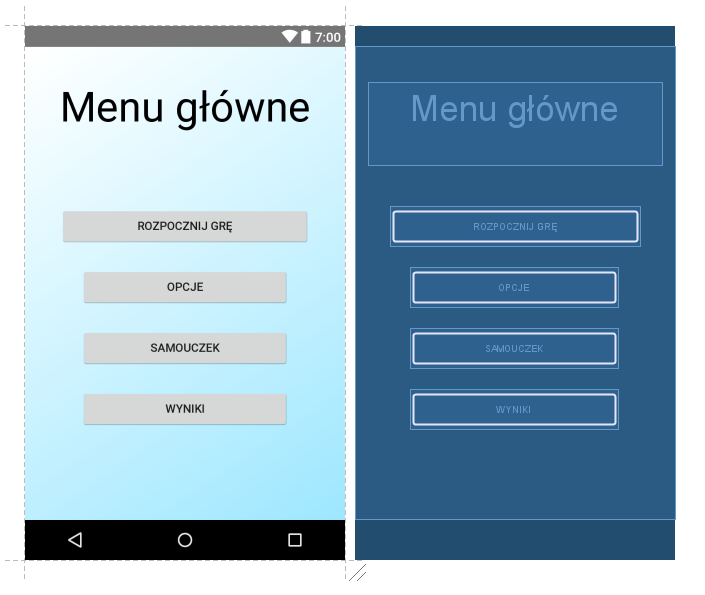
\includegraphics[scale=0.5]{amenu.png}
\end{center}
\caption{Projekt wygl�du menu g��wnego aplikacji.}
\label{amenu}
\end{figure}

\subsection{activity\_numbers}\label{numbers}
Widok pokazuj�cy wygl�d ca�ego testu pami�ci (Rys. \ref{anumbers}). Zawiera 10 przycisk�w odpowiedzialnych za wpisywanie cyfr. S� u�o�one w wygodny do u�ytkowania spos�b. Przyciski te s� oznaczone odpowiednim symbolem, przez co u�ytkownik wie, jaka cyfra pojawi si� po naci�ni�ciu na dan� kontrolk�. Do usuwania wpisywanego przez om�wione elementy ci�gu, s�u�y przycisk z wizerunkiem standardowego klawisza do usuwania tekstu w klawiaturach systemu Android. Kolejn� kontrolk� jest przycisk z napisem ,,GOT�W". S�u�y on do wyra�enia gotowo�ci i przej�cia do nast�pnego etapu rozgrywki. ImageButton, z wizerunkiem mikrofonu, s�u�y do w��czenia wprowadzania g�osowego.
\\ \indent
Widok zawiera dwa pola tekstowe. Pierwsze, na samej g�rze, s�u�y do informowania u�ytkownika o aktualnym etapie testu. W drugim, poni�ej, ukazuje si� ci�g do zapami�tania, wpisywana przez u�ytkownika zapami�tana sekwencja oraz statystyki po zako�czeniu rozgrywki. Dodatkowo, dooko�a drugiego pola tekstowego znajduje si� obramowanie. Wygl�d ramki zosta� utworzony w pliku frame.xlm opisanym w rozdziale \ref{frame}.
\\ \indent
W projekcie widoku niekt�re elementy nak�adaj� si� na siebie, jednak�e podczas testu, kontrolki zosta�y tak zaprogramowane, �e zmieniaj� swoje po�o�enie w zale�no�ci od danego etapu rozgrywki. Wszystko jest zaprojektowane w taki spos�b, by by�o jak najbardziej czytelne i intuicyjne dla u�ytkownika.

\begin{figure} [H]
\begin{center}
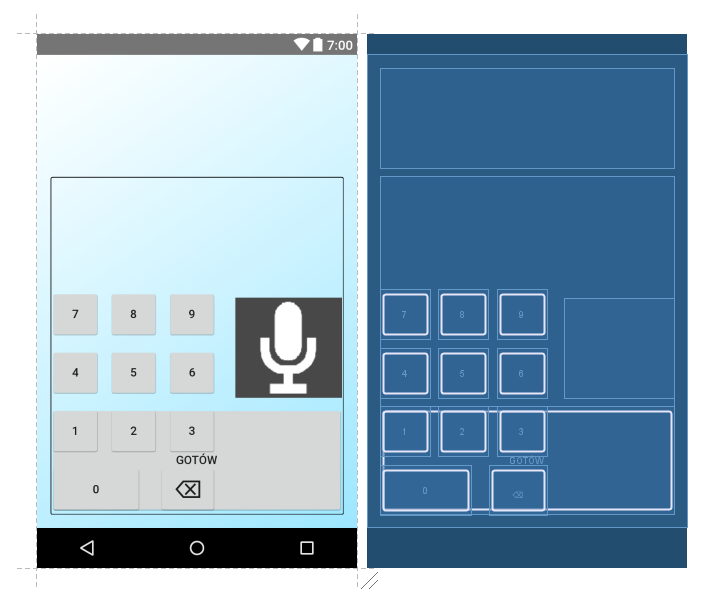
\includegraphics[scale=0.6]{anumbers.png}
\end{center}
\caption{Projekt wygl�du okna rozgrywki.}
\label{anumbers}
\end{figure}
\newpage
\subsection{activity\_options}
Okno opcji pokazuje dost�pn� mo�liwo�� konfiguracji (Rys. \ref{aoptions}). Trzy pola tekstowe informuj� u�ytkownika jakie ustawienia modyfikuje. Znajduj�ce si� przyciski pokazuj� swoim tekstem skutek zmiany danej opcji. Przesuni�cie suwaka zmienia pocz�tkow� d�ugo�� ci�gu. Jest on przesuwalny w warto�ciach od 0 do 49, jednak do wybranej warto�ci suwaka dodawana jest jedynka. Da to mo�liwo�� ustawienia pocz�tkowej d�ugo�ci ci�gu w zakresie od 1 do 50. Pole tekstowe, znajduj�ce si� nad suwakiem, wy�wietla zadan� warto�� pocz�tkowej d�ugo�ci sekwencji.

\begin{figure} [H]
\begin{center}
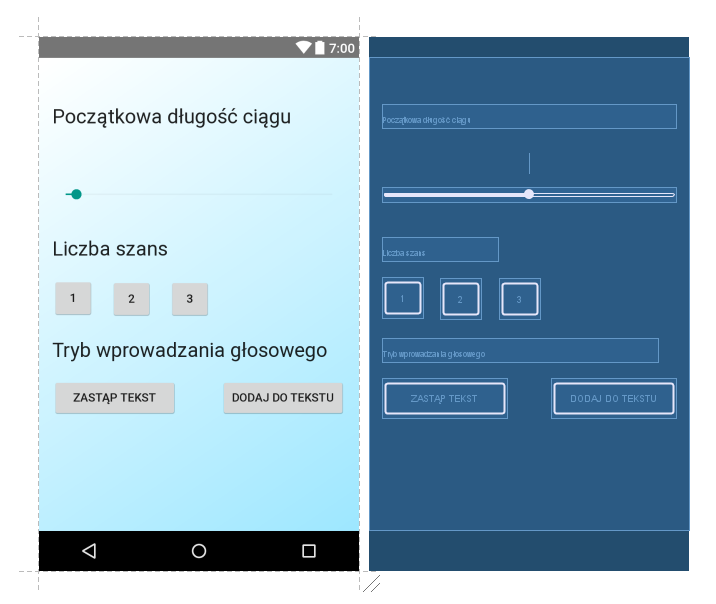
\includegraphics[scale=0.5]{aoptions.png}
\end{center}
\caption{Projekt wygl�du menu opcji.}
\label{aoptions}
\end{figure}

\subsection{activity\_results}
Jest to plik widoku, odpowiedzialny za wy�wietlenie wynik�w uko�czonych test�w. Informuje o tym pole tekstowe, znajduj�ce si� na samej g�rze okna. Poni�ej znajduje si� liniowy uk�ad horyzontalny, w sk�ad kt�rego wchodz� trzy pola tekstowe. Informuj� one o typie wy�wietlanej pod tekstem pozycji.
\\ \indent
W celu wy�wietlenia samych wynik�w, zosta�a dodana kontrolka ListView. Lista jest przewijalna i nieograniczona w ilo�ci pokazywanych element�w. W celu prawid�owego wy�wietlania ��danych wynik�w, zosta� dodany plik formatuj�cy pojedynczy wiersz listy. Zosta� on opisany w rozdziale \ref{listrow}.

\begin{figure} [H]
\begin{center}
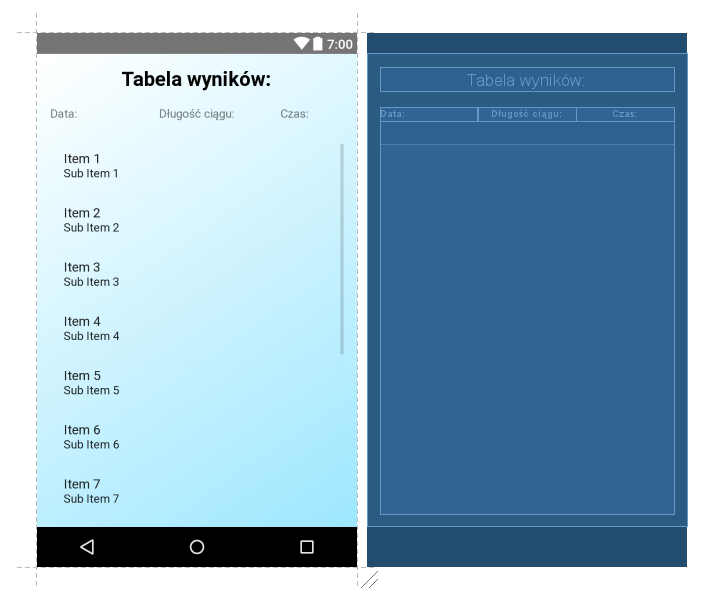
\includegraphics[scale=0.5]{aresults.png}
\end{center}
\caption{Projekt wygl�du listy wynik�w.}
\label{aresults}
\end{figure}

\subsection{list\_row}\label{listrow}
Uk�ad ustawiaj�cy wygl�d pojedynczego wierszu listy z wynikami. Jeden wiersz sk�ada si� z trzech p�l -- data wykonania testu, d�ugo�� zapami�tanego ci�gu oraz czas zapami�tywania najd�u�szej, poprawnie odtworzonej sekwencji. Pole z dat� jest odrobin� d�u�sze od pozosta�ych p�l. Zapobiega to zawijaniu si� tekstu w danym wierszu. 
\subsection{frame}\label{frame}
Plik zawiera styl ramki wok� pola tekstowego wy�wietlaj�cego np. ci�g cyfr do zapami�tania. Ramka jest koloru czarnego, ma lekko zaokr�glone rogi, a jej szeroko�� wynosi 1 dp (density independent pixel). T�o wn�trza ramki zosta�o ustawione na przezroczyste, aby nie zas�ania�o t�a ca�ego okna.
\subsection{gradient}
Odpowiedzialny jest za t�o ka�dego okna aplikacji. �rodowisko Android Studio umo�liwia w �atwy spos�b utworzenie gradientu o zadanych parametrach. Tak wygenerowany gradient nale�y za��czy� do ka�dego pliku z widokiem, gdzie przeskaluje si� na ca�e okno lub inny ��dany wymiar.
\newpage
\section{Klasy i metody}
Kod �r�d�owy aplikacji sk�ada si� z nast�puj�cych klas:
\begin{itemize}
\item Menu.java,
\item Numbers.java,
\item Tutorial.java,
\item Options.java,
\item Results.java,
\item MultirowLVAdapter.java.
\end{itemize}
Wa�nym plikiem jest r�wnie� plik AndroidManifest.xml, w kt�rym zawarte s� pozwolenia na zapis i odczyt danych z pami�ci urz�dzenia. Plik ten zawiera r�wnie� ustawienie pocz�tkowej aktywno�ci, uruchamianej zaraz po za��czeniu aplikacji. Dodatkowo okre�lona jest orientacja ekranu ka�dego z widok�w na ,,portrait'', co odpowiada pionowemu u�o�eniu telefonu.
\subsection{Menu}
Klasa obs�uguj�ca akcje wykonywane w menu g��wnym aplikacji. Pobiera kontrolki z widoku activity\_menu (Opisany w rozdziale \ref{menu}). Do przycisk�w przyporz�dkowana jest akcja rozpocz�cia odpowiadaj�cej przyciskowi aktywno�ci. Tak dla przyk�adu, po naci�ni�ciu klawiszu z napisem ,,Samouczek", poprzez metod� startActivity (metoda �rodowiska Android Studio), zostaje uruchomiona aktywno�� odpowiedzialna za samouczek.
\\ \indent
W tej aktywno�ci, poprzez metod� verifyStoragePermissions, wysy�ane jest ��danie o udzielenie pozwolenia na zapis i odczyt plik�w w pami�ci urz�dzenia. Na pocz�tku sprawdzane jest czy aplikacja ju� nie ma przyznanego pozwolenia. Je�eli nie ma, wysy�ane jest zapytanie, a je�li zezwolenie zosta�o przyznane, to nic nie robi. Taki zabieg umo�liwia pomini�cie wys�ania ��dania przy ka�dym uruchomieniu aplikacji, a nawet przy ka�dym wej�ciu do menu g��wnego.
\\ \indent 
Mimo, �e przyzwolenia na zapis i odczyt s� ju� przyznane w pliku AndroidManifest.xml, to dla nowszych wersji systemu Android (Android 6.0+), wymagane jest wy�wietlenie tej informacji u�ytkownikowi i zapytanie go o wyra�on� zgod�.
\subsection{Numbers}
Klasa obs�uguj�ca ca�y przebieg testu pami�ci kr�tkotrwa�ej. Pobiera on widok z pliku activity\_numbers.xml (Opisany w rozdziale \ref{numbers}). G��wnym elementem dzia�ania programu jest metoda onCreate, a dok�adniej nas�uchiwanie na naci�ni�cie przycisku z tagiem 'ok'. Po jego naci�ni�ciu, w zale�no�ci od etapu testu, uruchamiane s� odpowiednie metody. Aktualny etap rozgrywki zale�ny jest od warto�ci zmiennej steruj�cej 'steering'. Zmienna ta przyjmuje warto�ci 0, 1 lub 2. Pierwsza warto�� okre�la etap zapami�tywania ci�gu cyfr przez u�ytkownika. W tym etapie uruchamia si� pomiar czasu zapami�tywania. Generuje si� r�wnie� ci�g cyfr, po czym wy�wietlany jest na ekranie. Przy naci�ni�ciu na przycisk wyra�aj�cy gotowo��, pomiar czasu zapami�tywania zatrzymuje si�, zmieniany jest wygl�d okna aplikacji, oraz zmienna steruj�ca przyjmuje warto�� 1. Ta warto�� okre�la etap wpisywania zapami�tanej sekwencji. Po kolejnym przyci�ni�ciu, w zale�no�ci od tego, czy u�ytkownikowi zosta�y jeszcze szanse lub nie, zmienna steruj�ca przyjmuje warto�ci odpowiednio 0 lub 2. Warto�� 2 okre�la zako�czenie testu, gdzie po ponownym naci�ni�ciu na omawiany przycisk, aplikacja ,,wraca'' do menu g��wnego. Przy tym etapie rozgrywki wy�wietlana jest informacja o ko�cu gry oraz ukazywane s� statystyki -- najd�u�szy zapami�tany ci�g oraz czas jego zapami�tywania. Je�li u�ytkownikowi nie uda�o si� zapami�ta� �adnej sekwencji, Aplikacja wychwyci to i poinformuje u�ytkownika o tym wyj�tku.
\\ \indent
Wygenerowanie losowego ci�gu cyfr przebiega w metodzie random\_number. Przyjmuje ona parametr 'length', kt�ry odpowiada d�ugo�ci wylosowanej sekwencji. Zadeklarowana zostaje zmienna tablicowa typu int o rozmiarze r�wnym warto�ci przes�anego parametru. Nast�pnie, do ka�dej kom�rki tej�e tablicy zostaje wpisana losowa cyfra. Tak wygenerowany ci�g zostaje zwr�cony do dalszych dzia�a�.
\\ \indent
Kolejnym krokiem jest przekszta�cenie wygenerowanego ci�gu z formy tablicy liczb ca�kowitych do typu String. Dzieje si� to w metodzie intarray2string, kt�ra przyjmuje parametr typu int tablicowy. P�tla przechodzi po ka�dej kom�rce tablicy i dopisuje jej warto�� do napisu. Przekonwertowany ci�g jest zwracany do dalszego u�ytku. Zabieg ten jest konieczny przy bezproblemowym wy�wietleniu ci�gu w polu tekstowym oraz �atwym por�wnaniu warto�ci wpisanej przez u�ytkownika z zapami�tywan� sekwencj�.
\\ \indent
Metoda sprawdzaj�ca poprawno�� zapami�tanej sekwencji to metoda check. Przyjmuje ona dwie zmienne typu String. Jedna zawiera ci�g cyfr do zapami�tania, a druga warto�� wpisan� przez u�ytkownika po zapami�taniu. Funkcja sprawdza czy napisy s� sobie zbie�ne. Je�eli tak, u�ytkownikowi zostaje wy�wietlony stosowny komunikat. D�ugo�� sekwencji zostaje zwi�kszona o jeden, czas zapami�tywania zostaje zapisany a tak�e zmienna 'remembered' zostaje ustawiona na true. Zmienna ta jest typu bool i zawiera informacje o tym, czy u�ytkownik zapami�ta� jakikolwiek ci�g. Do tego etapu, zmienna ta jest ustawiona na false. Przy negatywnym wyniku por�wnania, zmniejszana jest liczba szans. Je�eli liczba szans jest wi�ksza od zera, u�ytkownikowi wy�wietlony jest komunikat o pozosta�ej liczbie szans. W przeciwnym przypadku, gracz zostaje poinformowany o zako�czeniu rozgrywki.
\\ \indent
Metoda odpowiedzialna za zmian� wygl�du aplikacji w zale�no�ci od aktualnego etapu testu pami�ci, to metoda invisibility......

\subsection{Tutorial}
\subsection{Options}
\subsection{Results}
\subsection{MultirowLVAdapter}

\chapter{Specyfikacja zewn�trzna}
\section{Menu g��wne}
\section{Rozgrywka}
\section{Samouczek}
\section{Opcje}
\section{Wyniki}

\chapter{Testy}
Tutaj w�a�nie efekt przetestowania aplikacji na grupie os�b: czy co� z tego wynika (od
opinii po wyniki numeryczne, zale�nie od tego, co uda si� zrobi�)

+ ewentualne uwagi: co warto rozwija� itp.
\chapter{Podsumowanie i wnioski}
Celem pracy by�o .... Zrobiono to, tamto i siamto. Cel pracy zosta� osi�gni�ty (lub nie0




  

%\appendix  % <--- zaczynaj� si� dodatki; jak nazywa si� rozdzia� -> szuka� appendixname powy�ej
%\chapter{Dodatek A}
W dodatku umieszczamy opis ewentualnych znanych algorytm�w, z kt�rych korzystamy proponuj�c w�asn� metodologi�, opisan� w rozdziale~\ref{Chapter_Metodologia}. Wykaz pozycji literaturowych tworzymy w oddzielnym pliku \texttt{Praca.bib}. Chc�c si� odwo�a� w tek�cie do wybranej pozycji bibliograficznej korzystamy z komendy \texttt{cite}. Efekt jej u�ycia dla kilku pozycji jednocze�nie to~\cite{Tadeusiewicz,Malina,Nieniewski_Morfologia}.

%%%%%%%%%%%%%%%%%%%%%%%%%%%%%%%%%%%%%%%%%%%%%%%%%%%%%%%%%%%%%%%%%%%%%%%%%%%%%%%%%%%%%%%%%%%%%%%%%%%%%%%%%%%%%%%%%%%%%%%%%%%%%%%%%%%%%%%%%%%%%%%%%%%%%%%%%%%%%%%%%%%%%%%
\chapter{Dodatek B}
Podstawowe kwestie techniczne dotycz�ce wzor�w, rysunk�w, tabel poni�ej.

Wzory tworzymy w �rodowisku \texttt{equation}. Chc�c odwo�a� si� do wybranego wzoru gdzie� w tek�cie nale�y nada� mu stosown�, niepowtarzaln� i jednoznaczn� etykiet�, po ty by m�c np. napisa� zdanie: ze wzoru~\ref{Wzor_Dodawanie} wynika \ldots
\begin{equation}\label{Wzor_Dodawanie}
	c = a + b
\end{equation}

Wzory z�o�one, charakteryzuj�ce si� przypisaniem warto�ci zmiennej w pewnych okoliczno�ciach tworzymy przy u�yciu otoczenia \texttt{eqnarray}. Odwo�anie do wzoru jak wcze�niej. 
\begin{eqnarray}\label{equ_progowanie}
    BW & = & \left \{
    \begin{array}{ll}
      1, & I(x,y) \geq T \\
      0, & I(x,y) < T\\
    \end{array}
    \right.,
\end{eqnarray}

% \subsection{Usuwanie numeracji przy r�wnaniach}

Numeracj� r�wna� mo�na tymczasowo (w~danej linijce) wy��czy� poprzez u�ycie $\backslash{}nonumber$
\begin{eqnarray}
	a_i = a_{i-1}+a_{i-2}\nonumber \\ % w tej linijce nie ma numeru
              +a_{i-3}
\end{eqnarray}


\section{Wstawianie rysunk�w}
Rysunki umieszczamy w otoczeniu \texttt{figure}, centruj�c je w poziomie komend� \texttt{centering}. Rozmiary rysunku ustalamy w komendzie \texttt{includegraphics} dobieraj�c wielko�� wzgl�dem rozmiaru strony lub bezwzgl�dnie np. w cm. Ponadto najpierw zapowiadamy pojawienie si� rysunku w tek�cie (czyli np. Na rysunku (Rys~\ref{Rysunek_LogoIB}) pracy, a dopiero p�niej wstawiamy sam rysunek. Dodatkowo sterowa� mo�emy umiejscowieniem rysunku na stronie dzi�ki parametrom \texttt{[!htb]} okre�laj�cym miejsce. Odpowiednio s� to: \texttt{here}, \texttt{top}, \texttt{bottom}. 
\begin{figure}[!htb]
	\centering
	
\includegraphics[width=.35\textwidth]{logoRIB}
	\caption{Logo Wydzia�u In�ynierii Biomedycznej.}\label{Rysunek_LogoIB}
\end{figure}

Do��czaj�c rysunki nie trzeba podawa� rozszerzenia (wr�cz jest to odradzane). Je�li rysunki znajduj� si� w~katalogu \emph{rysunki}, nie trzeba r�wnie� podawa� �cie�ki do nich.

\section{Wstawianie tabelek}
Analogicznie post�pujemy z tabelkami, z t� r�nic� �e tworzymy j� w otoczeniu \texttt{table}. W nim natomiast sam� tabel� definiujemy albo w �rodowisku \texttt{tabular}, albo \texttt{tabularx}. Podobnie z odwo�aniami w tek�cie: najpierw odwo�anie w Tab.~\ref{Tabelka_Tabela}, a dopiero p�niej sama tabela.
\begin{table}[!htb]
	\centering
	\topcaption{Opis nad tabelk�.}\label{Tabelka_Tabela}
	\begin{tabular}{|c|c|c|c|} \hline \hline 
		Kolumna 1 & Kolumna 2 & Kolumna 3 & Kolumna 4 \\ \hline
		Wiersz 1 & & & \\ \hline
		Wiersz 2 & & & \\ \hline
		Wiersz 3 & & & \\ \hline
		& & & \\ \hline
		& & & \\ \hline
	\end{tabular}
\end{table}

%%%%%%%%%%%%%%%%%%%%%%%%%%%%%%%%%%%%%%%%%%%%%%%%%%%%%%%%%%%%%%%%%%%%%%%%%%%%%%%%%%%%%%%%%%%%%%%%%%%%%%%%%%%%%%%%%%%%%%%%%%%%%%%%%%%%%%%%%%%%%%%%%%%%%%%%%%%%%%%%%%%%%%%
\chapter{Kwestie edytorskie}
Zbi�r zasad pomocnych przy redagowaniu tekstu pracy wystarczaj�co szczeg�owo przedstawia ksi��ka~\cite{Chwalowski}.

Uwaga! Pisz�c prac� nale�y zwr�ci� uwag� na nast�puj�ce kwestie:
\begin{enumerate}
	\item Prace piszemy w formie bezosobowej.
	\item Unikamy okre�le� potocznych, spolszcze� funkcjonuj�cych codziennej mowie itp.
	\item Pos�uguj�c si� znanymi nam (a nie czytelnikowi) has�ami (r�wnie� skr�tami, akronimami) najpierw je definiujemy i~t�umaczymy, a~dopiero p�niej traktujemy za znane.
	\item Podpisy pod rysunkami lub nad tabelami traktujemy jak zdania, a wi�c powinny stanowi� sp�jn� ca�o�� oraz powinny zosta� zako�czone kropk�.
	\item Podobnie wypunktowania (po dwukropku kolejne punkty pisane ma�ymi literami, oddzielane przecinkami, ostatni zako�czony kropk� o ile ko�czy zdanie).
	\item Do ka�dego rysunku, tabeli, pozycji bibliograficznej musi istnie� odwo�anie w tek�cie pracy, przy czym do pierwszych dw�ch musi si� ono pojawi� zanim umie�cimy rysunek/tabel�.
\end{enumerate}


\clearpage \addcontentsline{toc}{chapter}{\bibname}
\bibliography{Praca}


\end{document}
